\documentclass[1p]{elsarticle_modified}
%\bibliographystyle{elsarticle-num}

%\usepackage[colorlinks]{hyperref}
%\usepackage{abbrmath_seonhwa} %\Abb, \Ascr, \Acal ,\Abf, \Afrak
\usepackage{amsfonts}
\usepackage{amssymb}
\usepackage{amsmath}
\usepackage{amsthm}
\usepackage{scalefnt}
\usepackage{amsbsy}
\usepackage{kotex}
\usepackage{caption}
\usepackage{subfig}
\usepackage{color}
\usepackage{graphicx}
\usepackage{xcolor} %% white, black, red, green, blue, cyan, magenta, yellow
\usepackage{float}
\usepackage{setspace}
\usepackage{hyperref}

\usepackage{tikz}
\usetikzlibrary{arrows}

\usepackage{multirow}
\usepackage{array} % fixed length table
\usepackage{hhline}

%%%%%%%%%%%%%%%%%%%%%
\makeatletter
\renewcommand*\env@matrix[1][\arraystretch]{%
	\edef\arraystretch{#1}%
	\hskip -\arraycolsep
	\let\@ifnextchar\new@ifnextchar
	\array{*\c@MaxMatrixCols c}}
\makeatother %https://tex.stackexchange.com/questions/14071/how-can-i-increase-the-line-spacing-in-a-matrix
%%%%%%%%%%%%%%%

\usepackage[normalem]{ulem}

\newcommand{\msout}[1]{\ifmmode\text{\sout{\ensuremath{#1}}}\else\sout{#1}\fi}
%SOURCE: \msout is \stkout macro in https://tex.stackexchange.com/questions/20609/strikeout-in-math-mode

\newcommand{\cancel}[1]{
	\ifmmode
	{\color{red}\msout{#1}}
	\else
	{\color{red}\sout{#1}}
	\fi
}

\newcommand{\add}[1]{
	{\color{blue}\uwave{#1}}
}

\newcommand{\replace}[2]{
	\ifmmode
	{\color{red}\msout{#1}}{\color{blue}\uwave{#2}}
	\else
	{\color{red}\sout{#1}}{\color{blue}\uwave{#2}}
	\fi
}

\newcommand{\Sol}{\mathcal{S}} %segment
\newcommand{\D}{D} %diagram
\newcommand{\A}{\mathcal{A}} %arc


%%%%%%%%%%%%%%%%%%%%%%%%%%%%%5 test

\def\sl{\operatorname{\textup{SL}}(2,\Cbb)}
\def\psl{\operatorname{\textup{PSL}}(2,\Cbb)}
\def\quan{\mkern 1mu \triangleright \mkern 1mu}

\theoremstyle{definition}
\newtheorem{thm}{Theorem}[section]
\newtheorem{prop}[thm]{Proposition}
\newtheorem{lem}[thm]{Lemma}
\newtheorem{ques}[thm]{Question}
\newtheorem{cor}[thm]{Corollary}
\newtheorem{defn}[thm]{Definition}
\newtheorem{exam}[thm]{Example}
\newtheorem{rmk}[thm]{Remark}
\newtheorem{alg}[thm]{Algorithm}

\newcommand{\I}{\sqrt{-1}}
\begin{document}

%\begin{frontmatter}
%
%\title{Boundary parabolic representations of knots up to 8 crossings}
%
%%% Group authors per affiliation:
%\author{Yunhi Cho} 
%\address{Department of Mathematics, University of Seoul, Seoul, Korea}
%\ead{yhcho@uos.ac.kr}
%
%
%\author{Seonhwa Kim} %\fnref{s_kim}}
%\address{Center for Geometry and Physics, Institute for Basic Science, Pohang, 37673, Korea}
%\ead{ryeona17@ibs.re.kr}
%
%\author{Hyuk Kim}
%\address{Department of Mathematical Sciences, Seoul National University, Seoul 08826, Korea}
%\ead{hyukkim@snu.ac.kr}
%
%\author{Seokbeom Yoon}
%\address{Department of Mathematical Sciences, Seoul National University, Seoul, 08826,  Korea}
%\ead{sbyoon15@snu.ac.kr}
%
%\begin{abstract}
%We find all boundary parabolic representation of knots up to 8 crossings.
%
%\end{abstract}
%\begin{keyword}
%    \MSC[2010] 57M25 
%\end{keyword}
%
%\end{frontmatter}

%\linenumbers
%\tableofcontents
%
\newcommand\colored[1]{\textcolor{white}{\rule[-0.35ex]{0.8em}{1.4ex}}\kern-0.8em\color{red} #1}%
%\newcommand\colored[1]{\textcolor{white}{ #1}\kern-2.17ex	\textcolor{white}{ #1}\kern-1.81ex	\textcolor{white}{ #1}\kern-2.15ex\color{red}#1	}

{\Large $\underline{12a_{0148}~(K12a_{0148})}$}

\setlength{\tabcolsep}{10pt}
\renewcommand{\arraystretch}{1.6}
\vspace{1cm}\begin{tabular}{m{100pt}>{\centering\arraybackslash}m{274pt}}
\multirow{5}{120pt}{
	\centering
	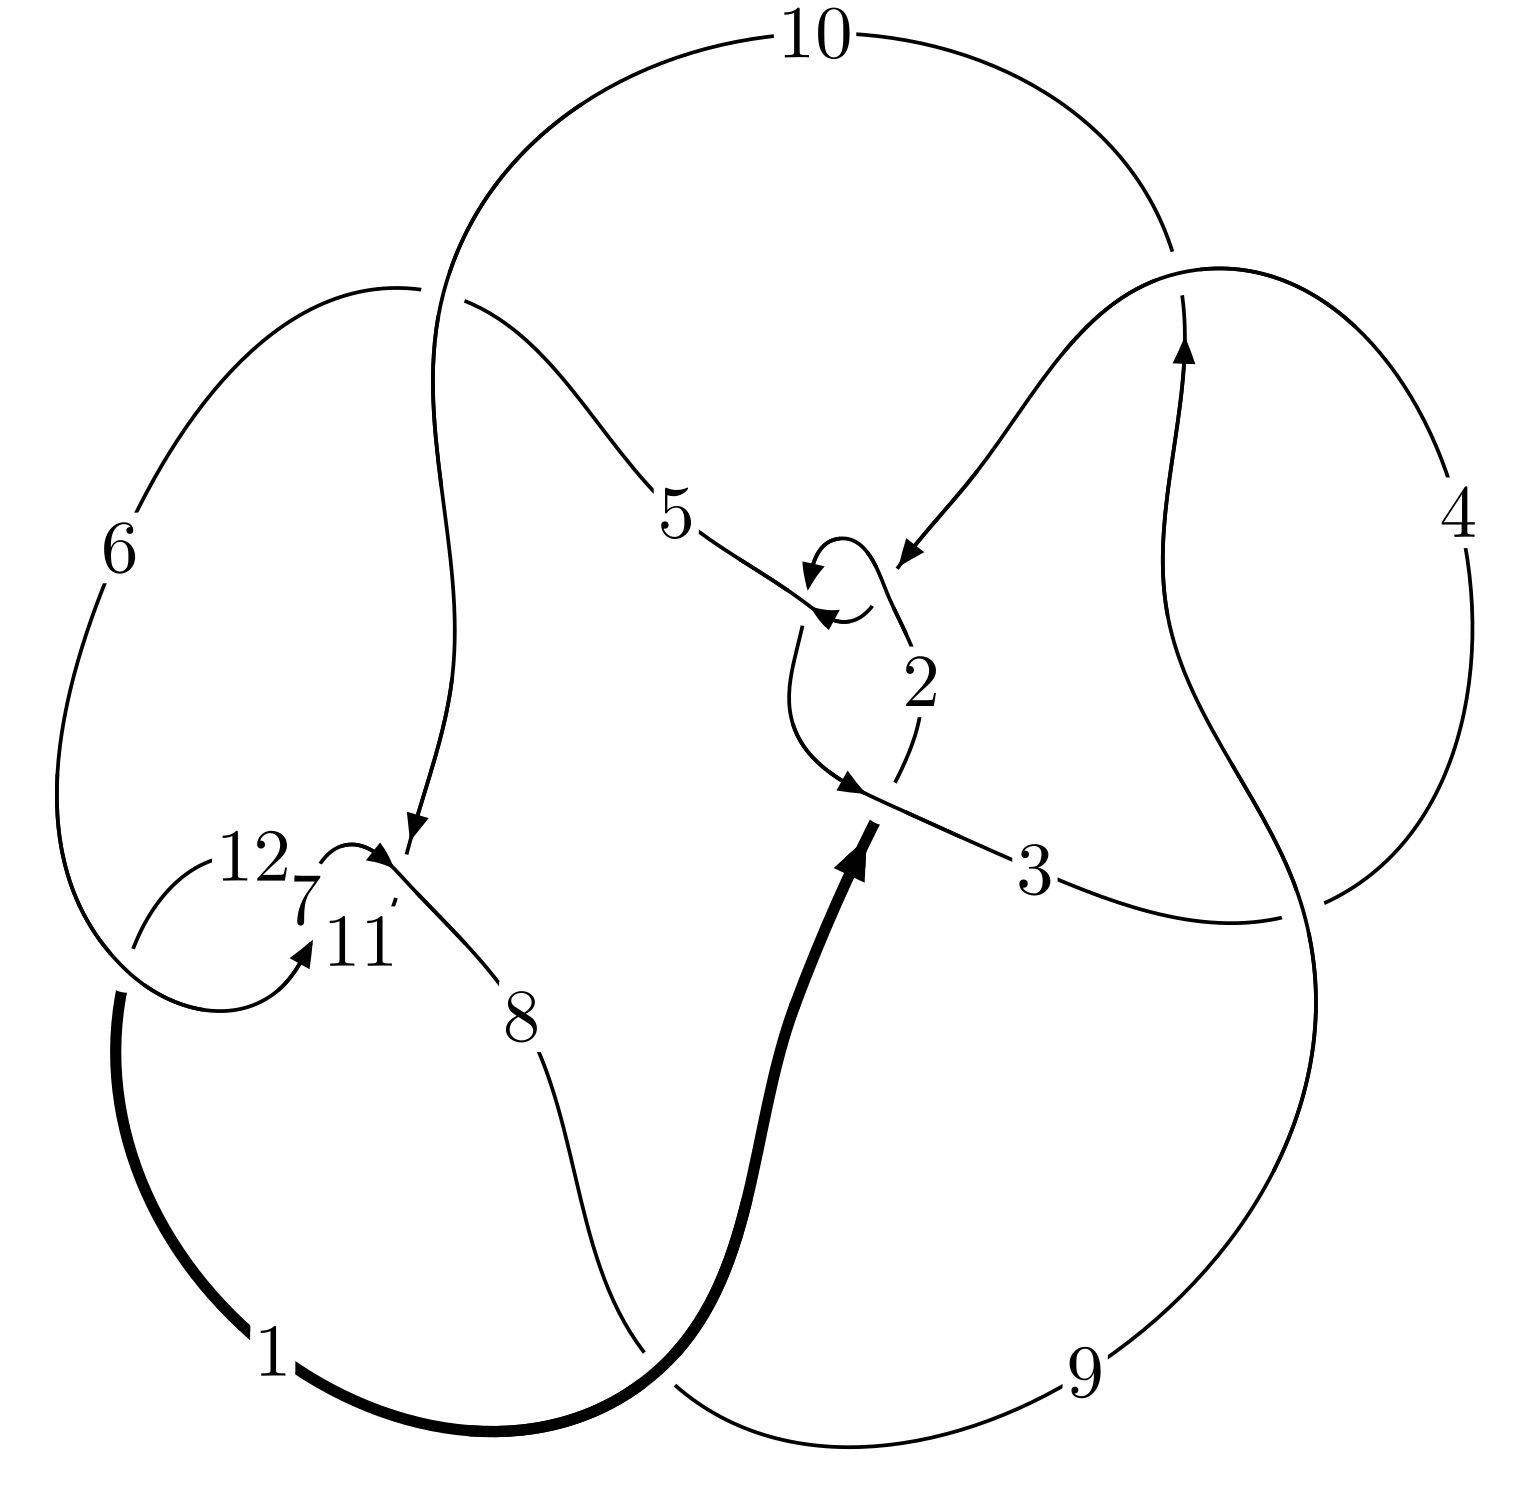
\includegraphics[width=112pt]{../../../GIT/diagram.site/Diagrams/png/949_12a_0148.png}\\
\ \ \ A knot diagram\footnotemark}&
\allowdisplaybreaks
\textbf{Linearized knot diagam} \\
\cline{2-2}
 &
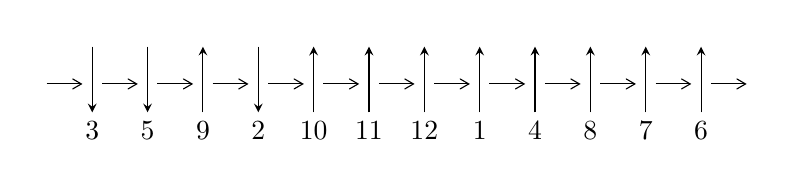
\begin{tikzpicture}[x=20pt, y=17pt]
	% nodes
	\node (C0) at (0, 0) {};
	\node (C1) at (1, 0) {};
	\node (C1U) at (1, +1) {};
	\node (C1D) at (1, -1) {3};

	\node (C2) at (2, 0) {};
	\node (C2U) at (2, +1) {};
	\node (C2D) at (2, -1) {5};

	\node (C3) at (3, 0) {};
	\node (C3U) at (3, +1) {};
	\node (C3D) at (3, -1) {9};

	\node (C4) at (4, 0) {};
	\node (C4U) at (4, +1) {};
	\node (C4D) at (4, -1) {2};

	\node (C5) at (5, 0) {};
	\node (C5U) at (5, +1) {};
	\node (C5D) at (5, -1) {10};

	\node (C6) at (6, 0) {};
	\node (C6U) at (6, +1) {};
	\node (C6D) at (6, -1) {11};

	\node (C7) at (7, 0) {};
	\node (C7U) at (7, +1) {};
	\node (C7D) at (7, -1) {12};

	\node (C8) at (8, 0) {};
	\node (C8U) at (8, +1) {};
	\node (C8D) at (8, -1) {1};

	\node (C9) at (9, 0) {};
	\node (C9U) at (9, +1) {};
	\node (C9D) at (9, -1) {4};

	\node (C10) at (10, 0) {};
	\node (C10U) at (10, +1) {};
	\node (C10D) at (10, -1) {8};

	\node (C11) at (11, 0) {};
	\node (C11U) at (11, +1) {};
	\node (C11D) at (11, -1) {7};

	\node (C12) at (12, 0) {};
	\node (C12U) at (12, +1) {};
	\node (C12D) at (12, -1) {6};
	\node (C13) at (13, 0) {};

	% arrows
	\draw[->,>={angle 60}]
	(C0) edge (C1) (C1) edge (C2) (C2) edge (C3) (C3) edge (C4) (C4) edge (C5) (C5) edge (C6) (C6) edge (C7) (C7) edge (C8) (C8) edge (C9) (C9) edge (C10) (C10) edge (C11) (C11) edge (C12) (C12) edge (C13) ;	\draw[->,>=stealth]
	(C1U) edge (C1D) (C2U) edge (C2D) (C3D) edge (C3U) (C4U) edge (C4D) (C5D) edge (C5U) (C6D) edge (C6U) (C7D) edge (C7U) (C8D) edge (C8U) (C9D) edge (C9U) (C10D) edge (C10U) (C11D) edge (C11U) (C12D) edge (C12U) ;
	\end{tikzpicture} \\
\hhline{~~} \\& 
\textbf{Solving Sequence} \\ \cline{2-2} 
 &
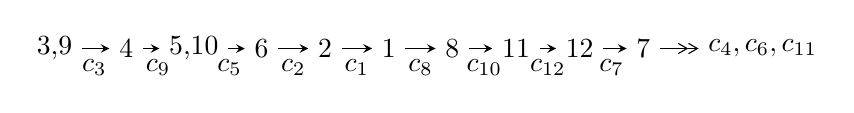
\begin{tikzpicture}[x=23pt, y=7pt]
	% node
	\node (A0) at (-1/8, 0) {3,9};
	\node (A1) at (1, 0) {4};
	\node (A2) at (33/16, 0) {5,10};
	\node (A3) at (25/8, 0) {6};
	\node (A4) at (33/8, 0) {2};
	\node (A5) at (41/8, 0) {1};
	\node (A6) at (49/8, 0) {8};
	\node (A7) at (57/8, 0) {11};
	\node (A8) at (65/8, 0) {12};
	\node (A9) at (73/8, 0) {7};
	\node (C1) at (1/2, -1) {$c_{3}$};
	\node (C2) at (3/2, -1) {$c_{9}$};
	\node (C3) at (21/8, -1) {$c_{5}$};
	\node (C4) at (29/8, -1) {$c_{2}$};
	\node (C5) at (37/8, -1) {$c_{1}$};
	\node (C6) at (45/8, -1) {$c_{8}$};
	\node (C7) at (53/8, -1) {$c_{10}$};
	\node (C8) at (61/8, -1) {$c_{12}$};
	\node (C9) at (69/8, -1) {$c_{7}$};
	\node (A10) at (11, 0) {$c_{4},c_{6},c_{11}$};

	% edge
	\draw[->,>=stealth]	
	(A0) edge (A1) (A1) edge (A2) (A2) edge (A3) (A3) edge (A4) (A4) edge (A5) (A5) edge (A6) (A6) edge (A7) (A7) edge (A8) (A8) edge (A9) ;
	\draw[->>,>={angle 60}]	
	(A9) edge (A10);
\end{tikzpicture} \\ 

\end{tabular} \\

\footnotetext{
The image of knot diagram is generated by the software ``\textbf{Draw programme}" developed by Andrew Bartholomew(\url{http://www.layer8.co.uk/maths/draw/index.htm\#Running-draw}), where we modified some parts for our purpose(\url{https://github.com/CATsTAILs/LinksPainter}).
}\phantom \\ \newline 
\centering \textbf{Ideals for irreducible components\footnotemark of $X_{\text{par}}$} 
 
\begin{align*}
I^u_{1}&=\langle 
4.42539\times10^{200} u^{87}-3.64946\times10^{199} u^{86}+\cdots+1.99958\times10^{199} b+9.22932\times10^{202},\\
\phantom{I^u_{1}}&\phantom{= \langle  }3.50341\times10^{201} u^{87}+1.47839\times10^{201} u^{86}+\cdots+1.59966\times10^{200} a+1.35973\times10^{204},\\
\phantom{I^u_{1}}&\phantom{= \langle  }u^{88}+u^{87}+\cdots+896 u+256\rangle \\
\\
I^v_{1}&=\langle 
a,\;b-1,\;v^8- v^7- v^6+2 v^5+v^4-2 v^3+2 v-1\rangle \\
\end{align*}
\raggedright * 2 irreducible components of $\dim_{\mathbb{C}}=0$, with total 96 representations.\\
\footnotetext{All coefficients of polynomials are rational numbers. But the coefficients are sometimes approximated in decimal forms when there is not enough margin.}
\newpage
\renewcommand{\arraystretch}{1}
\centering \section*{I. $I^u_{1}= \langle 4.43\times10^{200} u^{87}-3.65\times10^{199} u^{86}+\cdots+2.00\times10^{199} b+9.23\times10^{202},\;3.50\times10^{201} u^{87}+1.48\times10^{201} u^{86}+\cdots+1.60\times10^{200} a+1.36\times10^{204},\;u^{88}+u^{87}+\cdots+896 u+256 \rangle$}
\flushleft \textbf{(i) Arc colorings}\\
\begin{tabular}{m{7pt} m{180pt} m{7pt} m{180pt} }
\flushright $a_{3}=$&$\begin{pmatrix}1\\0\end{pmatrix}$ \\
\flushright $a_{9}=$&$\begin{pmatrix}0\\u\end{pmatrix}$ \\
\flushright $a_{4}=$&$\begin{pmatrix}1\\- u^2\end{pmatrix}$ \\
\flushright $a_{5}=$&$\begin{pmatrix}-21.9009 u^{87}-9.24189 u^{86}+\cdots-17882.8 u-8500.07\\-22.1316 u^{87}+1.82512 u^{86}+\cdots-13328.4 u-4615.63\end{pmatrix}$ \\
\flushright $a_{10}=$&$\begin{pmatrix}u\\- u^3+u\end{pmatrix}$ \\
\flushright $a_{6}=$&$\begin{pmatrix}-36.3315 u^{87}-7.56623 u^{86}+\cdots-26362.6 u-11326.7\\-20.1398 u^{87}+4.15579 u^{86}+\cdots-11071.2 u-3319.07\end{pmatrix}$ \\
\flushright $a_{2}=$&$\begin{pmatrix}-21.9009 u^{87}-9.24189 u^{86}+\cdots-17882.8 u-8500.07\\27.4223 u^{87}+3.72173 u^{86}+\cdots+19064.3 u+7856.34\end{pmatrix}$ \\
\flushright $a_{1}=$&$\begin{pmatrix}5.52139 u^{87}-5.52016 u^{86}+\cdots+1181.43 u-643.728\\27.4223 u^{87}+3.72173 u^{86}+\cdots+19064.3 u+7856.34\end{pmatrix}$ \\
\flushright $a_{8}=$&$\begin{pmatrix}-57.6042 u^{87}-9.93484 u^{86}+\cdots-40728.9 u-17176.4\\-9.77552 u^{87}+1.20789 u^{86}+\cdots-5709.00 u-1880.73\end{pmatrix}$ \\
\flushright $a_{11}=$&$\begin{pmatrix}10.1990 u^{87}-4.09790 u^{86}+\cdots+4767.62 u+1155.77\\-16.1258 u^{87}-3.46355 u^{86}+\cdots-11668.8 u-5093.69\end{pmatrix}$ \\
\flushright $a_{12}=$&$\begin{pmatrix}22.0367 u^{87}-6.36866 u^{86}+\cdots+11313.4 u+3063.28\\-4.70307 u^{87}-3.57832 u^{86}+\cdots-4496.61 u-2419.16\end{pmatrix}$ \\
\flushright $a_{7}=$&$\begin{pmatrix}-69.8135 u^{87}-16.6900 u^{86}+\cdots-51473.6 u-22702.9\\-35.6897 u^{87}+7.12445 u^{86}+\cdots-19702.9 u-5719.85\end{pmatrix}$\\&\end{tabular}
\flushleft \textbf{(ii) Obstruction class $= -1$}\\~\\
\flushleft \textbf{(iii) Cusp Shapes $= -61.0516 u^{87}-11.3428 u^{86}+\cdots-43625.8 u-18291.7$}\\~\\
\newpage\renewcommand{\arraystretch}{1}
\flushleft \textbf{(iv) u-Polynomials at the component}\newline \\
\begin{tabular}{m{50pt}|m{274pt}}
Crossings & \hspace{64pt}u-Polynomials at each crossing \\
\hline $$\begin{aligned}c_{1}\end{aligned}$$&$\begin{aligned}
&u^{88}+39 u^{87}+\cdots+48 u+1
\end{aligned}$\\
\hline $$\begin{aligned}c_{2},c_{4}\end{aligned}$$&$\begin{aligned}
&u^{88}-9 u^{87}+\cdots-16 u+1
\end{aligned}$\\
\hline $$\begin{aligned}c_{3},c_{9}\end{aligned}$$&$\begin{aligned}
&u^{88}- u^{87}+\cdots-896 u+256
\end{aligned}$\\
\hline $$\begin{aligned}c_{5},c_{8}\end{aligned}$$&$\begin{aligned}
&u^{88}+2 u^{87}+\cdots+7868 u+1960
\end{aligned}$\\
\hline $$\begin{aligned}c_{6},c_{7},c_{11}\end{aligned}$$&$\begin{aligned}
&u^{88}-2 u^{87}+\cdots+2 u^2+1
\end{aligned}$\\
\hline $$\begin{aligned}c_{10},c_{12}\end{aligned}$$&$\begin{aligned}
&u^{88}+6 u^{87}+\cdots+4 u+1
\end{aligned}$\\
\hline
\end{tabular}\\~\\
\newpage\renewcommand{\arraystretch}{1}
\flushleft \textbf{(v) Riley Polynomials at the component}\newline \\
\begin{tabular}{m{50pt}|m{274pt}}
Crossings & \hspace{64pt}Riley Polynomials at each crossing \\
\hline $$\begin{aligned}c_{1}\end{aligned}$$&$\begin{aligned}
&y^{88}+29 y^{87}+\cdots-2128 y+1
\end{aligned}$\\
\hline $$\begin{aligned}c_{2},c_{4}\end{aligned}$$&$\begin{aligned}
&y^{88}-39 y^{87}+\cdots-48 y+1
\end{aligned}$\\
\hline $$\begin{aligned}c_{3},c_{9}\end{aligned}$$&$\begin{aligned}
&y^{88}-51 y^{87}+\cdots-1949696 y+65536
\end{aligned}$\\
\hline $$\begin{aligned}c_{5},c_{8}\end{aligned}$$&$\begin{aligned}
&y^{88}-66 y^{87}+\cdots+35490896 y+3841600
\end{aligned}$\\
\hline $$\begin{aligned}c_{6},c_{7},c_{11}\end{aligned}$$&$\begin{aligned}
&y^{88}-74 y^{87}+\cdots+4 y+1
\end{aligned}$\\
\hline $$\begin{aligned}c_{10},c_{12}\end{aligned}$$&$\begin{aligned}
&y^{88}+46 y^{87}+\cdots+4 y+1
\end{aligned}$\\
\hline
\end{tabular}\\~\\
\newpage\flushleft \textbf{(vi) Complex Volumes and Cusp Shapes}
$$\begin{array}{c|c|c}  
\text{Solutions to }I^u_{1}& \I (\text{vol} + \sqrt{-1}CS) & \text{Cusp shape}\\
 \hline 
\begin{aligned}
u &= \phantom{-}1.00435\phantom{ +0.000000I} \\
a &= \phantom{-}0.429782\phantom{ +0.000000I} \\
b &= \phantom{-}1.32676\phantom{ +0.000000I}\end{aligned}
 & \phantom{-}6.57645\phantom{ +0.000000I} & \phantom{-0.000000 } 0 \\ \hline\begin{aligned}
u &= -1.001690 + 0.149224 I \\
a &= \phantom{-}0.429739 + 0.012969 I \\
b &= \phantom{-}1.324880 - 0.070161 I\end{aligned}
 & \phantom{-}2.39022 - 7.28873 I & \phantom{-0.000000 } 0 \\ \hline\begin{aligned}
u &= -1.001690 - 0.149224 I \\
a &= \phantom{-}0.429739 - 0.012969 I \\
b &= \phantom{-}1.324880 + 0.070161 I\end{aligned}
 & \phantom{-}2.39022 + 7.28873 I & \phantom{-0.000000 } 0 \\ \hline\begin{aligned}
u &= \phantom{-}0.957734 + 0.153558 I \\
a &= \phantom{-}0.433584 - 0.013510 I \\
b &= \phantom{-}1.304120 + 0.071792 I\end{aligned}
 & -2.38943 + 3.43455 I & \phantom{-0.000000 } 0 \\ \hline\begin{aligned}
u &= \phantom{-}0.957734 - 0.153558 I \\
a &= \phantom{-}0.433584 + 0.013510 I \\
b &= \phantom{-}1.304120 - 0.071792 I\end{aligned}
 & -2.38943 - 3.43455 I & \phantom{-0.000000 } 0 \\ \hline\begin{aligned}
u &= -0.219203 + 1.015630 I \\
a &= \phantom{-}0.500350 + 0.146984 I \\
b &= \phantom{-}0.839830 - 0.540473 I\end{aligned}
 & \phantom{-}1.67070 + 2.16357 I & \phantom{-0.000000 } 0 \\ \hline\begin{aligned}
u &= -0.219203 - 1.015630 I \\
a &= \phantom{-}0.500350 - 0.146984 I \\
b &= \phantom{-}0.839830 + 0.540473 I\end{aligned}
 & \phantom{-}1.67070 - 2.16357 I & \phantom{-0.000000 } 0 \\ \hline\begin{aligned}
u &= -1.031030 + 0.152271 I \\
a &= \phantom{-}0.58647 + 1.56663 I \\
b &= -0.790418 - 0.559855 I\end{aligned}
 & \phantom{-}1.37194 - 0.87864 I & \phantom{-0.000000 } 0 \\ \hline\begin{aligned}
u &= -1.031030 - 0.152271 I \\
a &= \phantom{-}0.58647 - 1.56663 I \\
b &= -0.790418 + 0.559855 I\end{aligned}
 & \phantom{-}1.37194 + 0.87864 I & \phantom{-0.000000 } 0 \\ \hline\begin{aligned}
u &= \phantom{-}0.098155 + 1.040920 I \\
a &= \phantom{-}0.515677 - 0.169679 I \\
b &= \phantom{-}0.749756 + 0.575742 I\end{aligned}
 & -0.582374 + 1.270130 I & \phantom{-0.000000 } 0\\
 \hline 
 \end{array}$$\newpage$$\begin{array}{c|c|c}  
\text{Solutions to }I^u_{1}& \I (\text{vol} + \sqrt{-1}CS) & \text{Cusp shape}\\
 \hline 
\begin{aligned}
u &= \phantom{-}0.098155 - 1.040920 I \\
a &= \phantom{-}0.515677 + 0.169679 I \\
b &= \phantom{-}0.749756 - 0.575742 I\end{aligned}
 & -0.582374 - 1.270130 I & \phantom{-0.000000 } 0 \\ \hline\begin{aligned}
u &= \phantom{-}0.576718 + 0.732950 I \\
a &= \phantom{-}0.466275 - 0.078251 I \\
b &= \phantom{-}1.085910 + 0.350059 I\end{aligned}
 & -1.59869 - 4.94887 I & \phantom{-0.000000 } 0 \\ \hline\begin{aligned}
u &= \phantom{-}0.576718 - 0.732950 I \\
a &= \phantom{-}0.466275 + 0.078251 I \\
b &= \phantom{-}1.085910 - 0.350059 I\end{aligned}
 & -1.59869 + 4.94887 I & \phantom{-0.000000 } 0 \\ \hline\begin{aligned}
u &= -0.305706 + 1.023880 I \\
a &= \phantom{-}0.486178 + 0.137784 I \\
b &= \phantom{-}0.903940 - 0.539582 I\end{aligned}
 & \phantom{-}1.49354 + 2.08175 I & \phantom{-0.000000 } 0 \\ \hline\begin{aligned}
u &= -0.305706 - 1.023880 I \\
a &= \phantom{-}0.486178 - 0.137784 I \\
b &= \phantom{-}0.903940 + 0.539582 I\end{aligned}
 & \phantom{-}1.49354 - 2.08175 I & \phantom{-0.000000 } 0 \\ \hline\begin{aligned}
u &= \phantom{-}0.977964 + 0.448688 I \\
a &= -0.00055 - 1.99302 I \\
b &= -1.000140 + 0.501752 I\end{aligned}
 & -0.69091 + 1.55122 I & \phantom{-0.000000 } 0 \\ \hline\begin{aligned}
u &= \phantom{-}0.977964 - 0.448688 I \\
a &= -0.00055 + 1.99302 I \\
b &= -1.000140 - 0.501752 I\end{aligned}
 & -0.69091 - 1.55122 I & \phantom{-0.000000 } 0 \\ \hline\begin{aligned}
u &= -0.087736 + 1.086640 I \\
a &= \phantom{-}0.509047 + 0.178283 I \\
b &= \phantom{-}0.749823 - 0.612838 I\end{aligned}
 & \phantom{-}4.24013 - 5.02346 I & \phantom{-0.000000 } 0 \\ \hline\begin{aligned}
u &= -0.087736 - 1.086640 I \\
a &= \phantom{-}0.509047 - 0.178283 I \\
b &= \phantom{-}0.749823 + 0.612838 I\end{aligned}
 & \phantom{-}4.24013 + 5.02346 I & \phantom{-0.000000 } 0 \\ \hline\begin{aligned}
u &= -0.601343 + 0.667675 I \\
a &= \phantom{-}0.464910 + 0.069332 I \\
b &= \phantom{-}1.104160 - 0.313793 I\end{aligned}
 & -5.59798 + 1.13427 I & \phantom{-0.000000 } 0\\
 \hline 
 \end{array}$$\newpage$$\begin{array}{c|c|c}  
\text{Solutions to }I^u_{1}& \I (\text{vol} + \sqrt{-1}CS) & \text{Cusp shape}\\
 \hline 
\begin{aligned}
u &= -0.601343 - 0.667675 I \\
a &= \phantom{-}0.464910 - 0.069332 I \\
b &= \phantom{-}1.104160 + 0.313793 I\end{aligned}
 & -5.59798 - 1.13427 I & \phantom{-0.000000 } 0 \\ \hline\begin{aligned}
u &= \phantom{-}0.647327 + 0.605586 I \\
a &= \phantom{-}0.460593 - 0.060958 I \\
b &= \phantom{-}1.133740 + 0.282394 I\end{aligned}
 & -1.76809 + 2.65293 I & \phantom{-0.000000 } 0 \\ \hline\begin{aligned}
u &= \phantom{-}0.647327 - 0.605586 I \\
a &= \phantom{-}0.460593 + 0.060958 I \\
b &= \phantom{-}1.133740 - 0.282394 I\end{aligned}
 & -1.76809 - 2.65293 I & \phantom{-0.000000 } 0 \\ \hline\begin{aligned}
u &= -1.007440 + 0.484362 I \\
a &= -0.08958 + 1.91917 I \\
b &= -1.024270 - 0.519926 I\end{aligned}
 & -4.28846 - 5.63711 I & \phantom{-0.000000 } 0 \\ \hline\begin{aligned}
u &= -1.007440 - 0.484362 I \\
a &= -0.08958 - 1.91917 I \\
b &= -1.024270 + 0.519926 I\end{aligned}
 & -4.28846 + 5.63711 I & \phantom{-0.000000 } 0 \\ \hline\begin{aligned}
u &= \phantom{-}1.096010 + 0.287738 I \\
a &= \phantom{-}0.28422 - 1.63973 I \\
b &= -0.897374 + 0.592068 I\end{aligned}
 & \phantom{-}1.01324 + 3.73408 I & \phantom{-0.000000 } 0 \\ \hline\begin{aligned}
u &= \phantom{-}1.096010 - 0.287738 I \\
a &= \phantom{-}0.28422 + 1.63973 I \\
b &= -0.897374 - 0.592068 I\end{aligned}
 & \phantom{-}1.01324 - 3.73408 I & \phantom{-0.000000 } 0 \\ \hline\begin{aligned}
u &= \phantom{-}0.213348 + 1.117470 I \\
a &= \phantom{-}0.487187 - 0.162434 I \\
b &= \phantom{-}0.847254 + 0.615896 I\end{aligned}
 & \phantom{-}8.14434 - 2.42174 I & \phantom{-0.000000 } 0 \\ \hline\begin{aligned}
u &= \phantom{-}0.213348 - 1.117470 I \\
a &= \phantom{-}0.487187 + 0.162434 I \\
b &= \phantom{-}0.847254 - 0.615896 I\end{aligned}
 & \phantom{-}8.14434 + 2.42174 I & \phantom{-0.000000 } 0 \\ \hline\begin{aligned}
u &= \phantom{-}0.322387 + 1.091330 I \\
a &= \phantom{-}0.476315 - 0.145185 I \\
b &= \phantom{-}0.920976 + 0.585529 I\end{aligned}
 & -1.11718 - 5.91216 I & \phantom{-0.000000 } 0\\
 \hline 
 \end{array}$$\newpage$$\begin{array}{c|c|c}  
\text{Solutions to }I^u_{1}& \I (\text{vol} + \sqrt{-1}CS) & \text{Cusp shape}\\
 \hline 
\begin{aligned}
u &= \phantom{-}0.322387 - 1.091330 I \\
a &= \phantom{-}0.476315 + 0.145185 I \\
b &= \phantom{-}0.920976 - 0.585529 I\end{aligned}
 & -1.11718 + 5.91216 I & \phantom{-0.000000 } 0 \\ \hline\begin{aligned}
u &= -0.859307\phantom{ +0.000000I} \\
a &= \phantom{-}0.442580\phantom{ +0.000000I} \\
b &= \phantom{-}1.25948\phantom{ +0.000000I}\end{aligned}
 & \phantom{-}0.232477\phantom{ +0.000000I} & \phantom{-}11.3810\phantom{ +0.000000I} \\ \hline\begin{aligned}
u &= -0.830025 + 0.174817 I \\
a &= \phantom{-}0.445016 + 0.015816 I \\
b &= \phantom{-}1.244270 - 0.079764 I\end{aligned}
 & \phantom{-}0.314091 + 0.198621 I & \phantom{-0.000000 } 0 \\ \hline\begin{aligned}
u &= -0.830025 - 0.174817 I \\
a &= \phantom{-}0.445016 - 0.015816 I \\
b &= \phantom{-}1.244270 + 0.079764 I\end{aligned}
 & \phantom{-}0.314091 - 0.198621 I & \phantom{-0.000000 } 0 \\ \hline\begin{aligned}
u &= \phantom{-}1.032070 + 0.514380 I \\
a &= -0.15414 - 1.85794 I \\
b &= -1.044350 + 0.534552 I\end{aligned}
 & -0.12676 + 9.73288 I & \phantom{-0.000000 } 0 \\ \hline\begin{aligned}
u &= \phantom{-}1.032070 - 0.514380 I \\
a &= -0.15414 + 1.85794 I \\
b &= -1.044350 - 0.534552 I\end{aligned}
 & -0.12676 - 9.73288 I & \phantom{-0.000000 } 0 \\ \hline\begin{aligned}
u &= -0.051824 + 0.840631 I \\
a &= \phantom{-}0.562713 + 0.136610 I \\
b &= \phantom{-}0.678195 - 0.407415 I\end{aligned}
 & \phantom{-}2.05221 + 1.93040 I & \phantom{-}6.00000 - 3.49207 I \\ \hline\begin{aligned}
u &= -0.051824 - 0.840631 I \\
a &= \phantom{-}0.562713 - 0.136610 I \\
b &= \phantom{-}0.678195 + 0.407415 I\end{aligned}
 & \phantom{-}2.05221 - 1.93040 I & \phantom{-}6.00000 + 3.49207 I \\ \hline\begin{aligned}
u &= -0.823823 + 0.171820 I \\
a &= \phantom{-}1.08150 + 2.00827 I \\
b &= -0.792131 - 0.385999 I\end{aligned}
 & \phantom{-}0.29466 - 2.12175 I & \phantom{-}6.00000 + 4.57537 I \\ \hline\begin{aligned}
u &= -0.823823 - 0.171820 I \\
a &= \phantom{-}1.08150 - 2.00827 I \\
b &= -0.792131 + 0.385999 I\end{aligned}
 & \phantom{-}0.29466 + 2.12175 I & \phantom{-}6.00000 - 4.57537 I\\
 \hline 
 \end{array}$$\newpage$$\begin{array}{c|c|c}  
\text{Solutions to }I^u_{1}& \I (\text{vol} + \sqrt{-1}CS) & \text{Cusp shape}\\
 \hline 
\begin{aligned}
u &= \phantom{-}1.164840 + 0.015673 I \\
a &= \phantom{-}0.519545 - 1.240270 I \\
b &= -0.712673 + 0.685914 I\end{aligned}
 & \phantom{-}6.62329 - 0.64955 I & \phantom{-0.000000 } 0 \\ \hline\begin{aligned}
u &= \phantom{-}1.164840 - 0.015673 I \\
a &= \phantom{-}0.519545 + 1.240270 I \\
b &= -0.712673 - 0.685914 I\end{aligned}
 & \phantom{-}6.62329 + 0.64955 I & \phantom{-0.000000 } 0 \\ \hline\begin{aligned}
u &= -0.322346 + 1.120770 I \\
a &= \phantom{-}0.472940 + 0.148909 I \\
b &= \phantom{-}0.923722 - 0.605700 I\end{aligned}
 & \phantom{-}3.70264 + 9.83487 I & \phantom{-0.000000 } 0 \\ \hline\begin{aligned}
u &= -0.322346 - 1.120770 I \\
a &= \phantom{-}0.472940 - 0.148909 I \\
b &= \phantom{-}0.923722 + 0.605700 I\end{aligned}
 & \phantom{-}3.70264 - 9.83487 I & \phantom{-0.000000 } 0 \\ \hline\begin{aligned}
u &= -0.691641 + 0.455798 I \\
a &= \phantom{-}0.853629 - 0.525545 I \\
b &= -0.150516 + 0.522993 I\end{aligned}
 & \phantom{-}1.87270 - 5.60259 I & \phantom{-}6.00000 + 6.15186 I \\ \hline\begin{aligned}
u &= -0.691641 - 0.455798 I \\
a &= \phantom{-}0.853629 + 0.525545 I \\
b &= -0.150516 - 0.522993 I\end{aligned}
 & \phantom{-}1.87270 + 5.60259 I & \phantom{-}6.00000 - 6.15186 I \\ \hline\begin{aligned}
u &= \phantom{-}0.776541 + 0.121597 I \\
a &= \phantom{-}1.41349 - 1.89153 I \\
b &= -0.746497 + 0.339237 I\end{aligned}
 & -2.93128 - 1.87221 I & \phantom{-}6.00000 + 0. I\phantom{ +0.000000I} \\ \hline\begin{aligned}
u &= \phantom{-}0.776541 - 0.121597 I \\
a &= \phantom{-}1.41349 + 1.89153 I \\
b &= -0.746497 - 0.339237 I\end{aligned}
 & -2.93128 + 1.87221 I & \phantom{-}6.00000 + 0. I\phantom{ +0.000000I} \\ \hline\begin{aligned}
u &= -0.735694 + 0.094036 I \\
a &= \phantom{-}1.70267 + 1.78739 I \\
b &= -0.720592 - 0.293311 I\end{aligned}
 & \phantom{-}1.54881 + 5.88294 I & \phantom{-}11.49151 - 1.84085 I \\ \hline\begin{aligned}
u &= -0.735694 - 0.094036 I \\
a &= \phantom{-}1.70267 - 1.78739 I \\
b &= -0.720592 + 0.293311 I\end{aligned}
 & \phantom{-}1.54881 - 5.88294 I & \phantom{-}11.49151 + 1.84085 I\\
 \hline 
 \end{array}$$\newpage$$\begin{array}{c|c|c}  
\text{Solutions to }I^u_{1}& \I (\text{vol} + \sqrt{-1}CS) & \text{Cusp shape}\\
 \hline 
\begin{aligned}
u &= -1.226590 + 0.300164 I \\
a &= \phantom{-}0.16868 + 1.45270 I \\
b &= -0.921134 - 0.679217 I\end{aligned}
 & \phantom{-}6.02695 - 5.91537 I & \phantom{-0.000000 } 0 \\ \hline\begin{aligned}
u &= -1.226590 - 0.300164 I \\
a &= \phantom{-}0.16868 - 1.45270 I \\
b &= -0.921134 + 0.679217 I\end{aligned}
 & \phantom{-}6.02695 + 5.91537 I & \phantom{-0.000000 } 0 \\ \hline\begin{aligned}
u &= \phantom{-}0.569700 + 0.462149 I \\
a &= \phantom{-}0.874864 + 0.418521 I \\
b &= -0.069835 - 0.444976 I\end{aligned}
 & -2.39619 + 1.83979 I & \phantom{-}5.06407 - 4.03961 I \\ \hline\begin{aligned}
u &= \phantom{-}0.569700 - 0.462149 I \\
a &= \phantom{-}0.874864 - 0.418521 I \\
b &= -0.069835 + 0.444976 I\end{aligned}
 & -2.39619 - 1.83979 I & \phantom{-}5.06407 + 4.03961 I \\ \hline\begin{aligned}
u &= -0.427991 + 0.540581 I \\
a &= \phantom{-}0.816176 - 0.306811 I \\
b &= \phantom{-}0.073526 + 0.403552 I\end{aligned}
 & \phantom{-}1.16464 + 1.76346 I & \phantom{-}8.83454 + 0.17315 I \\ \hline\begin{aligned}
u &= -0.427991 - 0.540581 I \\
a &= \phantom{-}0.816176 + 0.306811 I \\
b &= \phantom{-}0.073526 - 0.403552 I\end{aligned}
 & \phantom{-}1.16464 - 1.76346 I & \phantom{-}8.83454 - 0.17315 I \\ \hline\begin{aligned}
u &= \phantom{-}1.301580 + 0.388579 I \\
a &= \phantom{-}0.479272 + 0.832451 I \\
b &= -0.480564 - 0.902214 I\end{aligned}
 & \phantom{-}6.52418 + 2.29472 I & \phantom{-0.000000 } 0 \\ \hline\begin{aligned}
u &= \phantom{-}1.301580 - 0.388579 I \\
a &= \phantom{-}0.479272 - 0.832451 I \\
b &= -0.480564 + 0.902214 I\end{aligned}
 & \phantom{-}6.52418 - 2.29472 I & \phantom{-0.000000 } 0 \\ \hline\begin{aligned}
u &= \phantom{-}1.320800 + 0.324605 I \\
a &= \phantom{-}0.463895 + 0.875320 I \\
b &= -0.527305 - 0.891925 I\end{aligned}
 & \phantom{-}6.81647 + 2.12430 I & \phantom{-0.000000 } 0 \\ \hline\begin{aligned}
u &= \phantom{-}1.320800 - 0.324605 I \\
a &= \phantom{-}0.463895 - 0.875320 I \\
b &= -0.527305 + 0.891925 I\end{aligned}
 & \phantom{-}6.81647 - 2.12430 I & \phantom{-0.000000 } 0\\
 \hline 
 \end{array}$$\newpage$$\begin{array}{c|c|c}  
\text{Solutions to }I^u_{1}& \I (\text{vol} + \sqrt{-1}CS) & \text{Cusp shape}\\
 \hline 
\begin{aligned}
u &= -1.357440 + 0.262000 I \\
a &= \phantom{-}0.430943 - 0.915034 I \\
b &= -0.578746 + 0.894462 I\end{aligned}
 & \phantom{-}4.81467 + 1.57988 I & \phantom{-0.000000 } 0 \\ \hline\begin{aligned}
u &= -1.357440 - 0.262000 I \\
a &= \phantom{-}0.430943 + 0.915034 I \\
b &= -0.578746 - 0.894462 I\end{aligned}
 & \phantom{-}4.81467 - 1.57988 I & \phantom{-0.000000 } 0 \\ \hline\begin{aligned}
u &= -1.327820 + 0.430064 I \\
a &= \phantom{-}0.462500 - 0.806106 I \\
b &= -0.464521 + 0.933303 I\end{aligned}
 & \phantom{-}4.02843 - 6.29523 I & \phantom{-0.000000 } 0 \\ \hline\begin{aligned}
u &= -1.327820 - 0.430064 I \\
a &= \phantom{-}0.462500 + 0.806106 I \\
b &= -0.464521 - 0.933303 I\end{aligned}
 & \phantom{-}4.02843 + 6.29523 I & \phantom{-0.000000 } 0 \\ \hline\begin{aligned}
u &= \phantom{-}0.601538\phantom{ +0.000000I} \\
a &= \phantom{-}1.84428\phantom{ +0.000000I} \\
b &= -0.457784\phantom{ +0.000000I}\end{aligned}
 & \phantom{-}5.87336\phantom{ +0.000000I} & \phantom{-}17.3130\phantom{ +0.000000I} \\ \hline\begin{aligned}
u &= -1.29156 + 0.57696 I \\
a &= -0.20838 + 1.42034 I \\
b &= -1.101120 - 0.689224 I\end{aligned}
 & \phantom{-}5.07279 - 7.95878 I & \phantom{-0.000000 } 0 \\ \hline\begin{aligned}
u &= -1.29156 - 0.57696 I \\
a &= -0.20838 - 1.42034 I \\
b &= -1.101120 + 0.689224 I\end{aligned}
 & \phantom{-}5.07279 + 7.95878 I & \phantom{-0.000000 } 0 \\ \hline\begin{aligned}
u &= \phantom{-}1.31363 + 0.52509 I \\
a &= -0.143157 - 1.398570 I \\
b &= -1.072430 + 0.707601 I\end{aligned}
 & \phantom{-}3.30771 + 4.32222 I & \phantom{-0.000000 } 0 \\ \hline\begin{aligned}
u &= \phantom{-}1.31363 - 0.52509 I \\
a &= -0.143157 + 1.398570 I \\
b &= -1.072430 - 0.707601 I\end{aligned}
 & \phantom{-}3.30771 - 4.32222 I & \phantom{-0.000000 } 0 \\ \hline\begin{aligned}
u &= -1.27396 + 0.62381 I \\
a &= -0.26980 + 1.43160 I \\
b &= -1.127130 - 0.674560 I\end{aligned}
 & \phantom{-}4.55871 - 8.10417 I & \phantom{-0.000000 } 0\\
 \hline 
 \end{array}$$\newpage$$\begin{array}{c|c|c}  
\text{Solutions to }I^u_{1}& \I (\text{vol} + \sqrt{-1}CS) & \text{Cusp shape}\\
 \hline 
\begin{aligned}
u &= -1.27396 - 0.62381 I \\
a &= -0.26980 - 1.43160 I \\
b &= -1.127130 + 0.674560 I\end{aligned}
 & \phantom{-}4.55871 + 8.10417 I & \phantom{-0.000000 } 0 \\ \hline\begin{aligned}
u &= \phantom{-}1.39560 + 0.25845 I \\
a &= \phantom{-}0.404256 + 0.910869 I \\
b &= -0.592938 - 0.917193 I\end{aligned}
 & \phantom{-}9.80224 - 5.29054 I & \phantom{-0.000000 } 0 \\ \hline\begin{aligned}
u &= \phantom{-}1.39560 - 0.25845 I \\
a &= \phantom{-}0.404256 - 0.910869 I \\
b &= -0.592938 + 0.917193 I\end{aligned}
 & \phantom{-}9.80224 + 5.29054 I & \phantom{-0.000000 } 0 \\ \hline\begin{aligned}
u &= \phantom{-}1.34834 + 0.44357 I \\
a &= \phantom{-}0.450169 + 0.798043 I \\
b &= -0.463781 - 0.950589 I\end{aligned}
 & \phantom{-}8.92156 + 10.27380 I & \phantom{-0.000000 } 0 \\ \hline\begin{aligned}
u &= \phantom{-}1.34834 - 0.44357 I \\
a &= \phantom{-}0.450169 - 0.798043 I \\
b &= -0.463781 + 0.950589 I\end{aligned}
 & \phantom{-}8.92156 - 10.27380 I & \phantom{-0.000000 } 0 \\ \hline\begin{aligned}
u &= -1.38667 + 0.36184 I \\
a &= \phantom{-}0.423626 - 0.845767 I \\
b &= -0.526559 + 0.945222 I\end{aligned}
 & \phantom{-}13.55820 - 2.57088 I & \phantom{-0.000000 } 0 \\ \hline\begin{aligned}
u &= -1.38667 - 0.36184 I \\
a &= \phantom{-}0.423626 + 0.845767 I \\
b &= -0.526559 - 0.945222 I\end{aligned}
 & \phantom{-}13.55820 + 2.57088 I & \phantom{-0.000000 } 0 \\ \hline\begin{aligned}
u &= \phantom{-}0.231987 + 0.508335 I \\
a &= \phantom{-}0.516989 - 0.041592 I \\
b &= \phantom{-}0.921836 + 0.154614 I\end{aligned}
 & -1.61463 - 0.56356 I & -2.54529 + 2.25978 I \\ \hline\begin{aligned}
u &= \phantom{-}0.231987 - 0.508335 I \\
a &= \phantom{-}0.516989 + 0.041592 I \\
b &= \phantom{-}0.921836 - 0.154614 I\end{aligned}
 & -1.61463 + 0.56356 I & -2.54529 - 2.25978 I \\ \hline\begin{aligned}
u &= \phantom{-}1.28815 + 0.64947 I \\
a &= -0.29632 - 1.40690 I \\
b &= -1.143350 + 0.680591 I\end{aligned}
 & \phantom{-}1.95879 + 12.20550 I & \phantom{-0.000000 } 0\\
 \hline 
 \end{array}$$\newpage$$\begin{array}{c|c|c}  
\text{Solutions to }I^u_{1}& \I (\text{vol} + \sqrt{-1}CS) & \text{Cusp shape}\\
 \hline 
\begin{aligned}
u &= \phantom{-}1.28815 - 0.64947 I \\
a &= -0.29632 + 1.40690 I \\
b &= -1.143350 - 0.680591 I\end{aligned}
 & \phantom{-}1.95879 - 12.20550 I & \phantom{-0.000000 } 0 \\ \hline\begin{aligned}
u &= -1.34931 + 0.52189 I \\
a &= -0.138486 + 1.357150 I \\
b &= -1.074410 - 0.729244 I\end{aligned}
 & \phantom{-}8.33102 - 0.74805 I & \phantom{-0.000000 } 0 \\ \hline\begin{aligned}
u &= -1.34931 - 0.52189 I \\
a &= -0.138486 - 1.357150 I \\
b &= -1.074410 + 0.729244 I\end{aligned}
 & \phantom{-}8.33102 + 0.74805 I & \phantom{-0.000000 } 0 \\ \hline\begin{aligned}
u &= -1.30005 + 0.66027 I \\
a &= -0.30494 + 1.38969 I \\
b &= -1.150650 - 0.686528 I\end{aligned}
 & \phantom{-}6.8211 - 16.2526 I & \phantom{-0.000000 } 0 \\ \hline\begin{aligned}
u &= -1.30005 - 0.66027 I \\
a &= -0.30494 - 1.38969 I \\
b &= -1.150650 + 0.686528 I\end{aligned}
 & \phantom{-}6.8211 + 16.2526 I & \phantom{-0.000000 } 0 \\ \hline\begin{aligned}
u &= \phantom{-}1.33561 + 0.60551 I \\
a &= -0.233965 - 1.363710 I \\
b &= -1.122210 + 0.712327 I\end{aligned}
 & \phantom{-}11.7348 + 8.6310 I & \phantom{-0.000000 } 0 \\ \hline\begin{aligned}
u &= \phantom{-}1.33561 - 0.60551 I \\
a &= -0.233965 + 1.363710 I \\
b &= -1.122210 - 0.712327 I\end{aligned}
 & \phantom{-}11.7348 - 8.6310 I & \phantom{-0.000000 } 0 \\ \hline\begin{aligned}
u &= -0.381782\phantom{ +0.000000I} \\
a &= \phantom{-}1.17518\phantom{ +0.000000I} \\
b &= -0.149070\phantom{ +0.000000I}\end{aligned}
 & \phantom{-}0.622395\phantom{ +0.000000I} & \phantom{-}16.0480\phantom{ +0.000000I}\\
 \hline 
 \end{array}$$\newpage\newpage\renewcommand{\arraystretch}{1}
\centering \section*{II. $I^v_{1}= \langle a,\;b-1,\;v^8- v^7- v^6+2 v^5+v^4-2 v^3+2 v-1 \rangle$}
\flushleft \textbf{(i) Arc colorings}\\
\begin{tabular}{m{7pt} m{180pt} m{7pt} m{180pt} }
\flushright $a_{3}=$&$\begin{pmatrix}1\\0\end{pmatrix}$ \\
\flushright $a_{9}=$&$\begin{pmatrix}v\\0\end{pmatrix}$ \\
\flushright $a_{4}=$&$\begin{pmatrix}1\\0\end{pmatrix}$ \\
\flushright $a_{5}=$&$\begin{pmatrix}0\\1\end{pmatrix}$ \\
\flushright $a_{10}=$&$\begin{pmatrix}v\\0\end{pmatrix}$ \\
\flushright $a_{6}=$&$\begin{pmatrix}v^2\\1\end{pmatrix}$ \\
\flushright $a_{2}=$&$\begin{pmatrix}1\\-1\end{pmatrix}$ \\
\flushright $a_{1}=$&$\begin{pmatrix}0\\-1\end{pmatrix}$ \\
\flushright $a_{8}=$&$\begin{pmatrix}v\\v\end{pmatrix}$ \\
\flushright $a_{11}=$&$\begin{pmatrix}- v^3+v\\- v^3\end{pmatrix}$ \\
\flushright $a_{12}=$&$\begin{pmatrix}v^4\\v^2-1\end{pmatrix}$ \\
\flushright $a_{7}=$&$\begin{pmatrix}- v^7+v^6+2 v^5- v^4-2 v^3+2 v^2+2 v-1\\- v^7+2 v^5-2 v^3+2 v\end{pmatrix}$\\&\end{tabular}
\flushleft \textbf{(ii) Obstruction class $= 1$}\\~\\
\flushleft \textbf{(iii) Cusp Shapes $= 2 v^7+v^6-5 v^5+v^4+4 v^3-2 v^2-2 v+6$}\\~\\
\newpage\renewcommand{\arraystretch}{1}
\flushleft \textbf{(iv) u-Polynomials at the component}\newline \\
\begin{tabular}{m{50pt}|m{274pt}}
Crossings & \hspace{64pt}u-Polynomials at each crossing \\
\hline $$\begin{aligned}c_{1},c_{2}\end{aligned}$$&$\begin{aligned}
&(u-1)^8
\end{aligned}$\\
\hline $$\begin{aligned}c_{3},c_{9}\end{aligned}$$&$\begin{aligned}
&u^8
\end{aligned}$\\
\hline $$\begin{aligned}c_{4}\end{aligned}$$&$\begin{aligned}
&(u+1)^8
\end{aligned}$\\
\hline $$\begin{aligned}c_{5},c_{8}\end{aligned}$$&$\begin{aligned}
&u^8+u^7- u^6-2 u^5+u^4+2 u^3-2 u-1
\end{aligned}$\\
\hline $$\begin{aligned}c_{6},c_{7}\end{aligned}$$&$\begin{aligned}
&u^8- u^7-3 u^6+2 u^5+3 u^4-2 u-1
\end{aligned}$\\
\hline $$\begin{aligned}c_{10},c_{12}\end{aligned}$$&$\begin{aligned}
&u^8-3 u^7+7 u^6-10 u^5+11 u^4-10 u^3+6 u^2-4 u+1
\end{aligned}$\\
\hline $$\begin{aligned}c_{11}\end{aligned}$$&$\begin{aligned}
&u^8+u^7-3 u^6-2 u^5+3 u^4+2 u-1
\end{aligned}$\\
\hline
\end{tabular}\\~\\
\newpage\renewcommand{\arraystretch}{1}
\flushleft \textbf{(v) Riley Polynomials at the component}\newline \\
\begin{tabular}{m{50pt}|m{274pt}}
Crossings & \hspace{64pt}Riley Polynomials at each crossing \\
\hline $$\begin{aligned}c_{1},c_{2},c_{4}\end{aligned}$$&$\begin{aligned}
&(y-1)^8
\end{aligned}$\\
\hline $$\begin{aligned}c_{3},c_{9}\end{aligned}$$&$\begin{aligned}
&y^8
\end{aligned}$\\
\hline $$\begin{aligned}c_{5},c_{8}\end{aligned}$$&$\begin{aligned}
&y^8-3 y^7+7 y^6-10 y^5+11 y^4-10 y^3+6 y^2-4 y+1
\end{aligned}$\\
\hline $$\begin{aligned}c_{6},c_{7},c_{11}\end{aligned}$$&$\begin{aligned}
&y^8-7 y^7+19 y^6-22 y^5+3 y^4+14 y^3-6 y^2-4 y+1
\end{aligned}$\\
\hline $$\begin{aligned}c_{10},c_{12}\end{aligned}$$&$\begin{aligned}
&y^8+5 y^7+11 y^6+6 y^5-17 y^4-34 y^3-22 y^2-4 y+1
\end{aligned}$\\
\hline
\end{tabular}\\~\\
\newpage\flushleft \textbf{(vi) Complex Volumes and Cusp Shapes}
$$\begin{array}{c|c|c}  
\text{Solutions to }I^v_{1}& \I (\text{vol} + \sqrt{-1}CS) & \text{Cusp shape}\\
 \hline 
\begin{aligned}
v &= \phantom{-}0.570868 + 0.730671 I \\
a &= \phantom{-0.000000 } 0 \\
b &= \phantom{-}1.00000\phantom{ +0.000000I}\end{aligned}
 & -0.604279 - 1.131230 I & \phantom{-}3.90459 + 0.80511 I \\ \hline\begin{aligned}
v &= \phantom{-}0.570868 - 0.730671 I \\
a &= \phantom{-0.000000 } 0 \\
b &= \phantom{-}1.00000\phantom{ +0.000000I}\end{aligned}
 & -0.604279 + 1.131230 I & \phantom{-}3.90459 - 0.80511 I \\ \hline\begin{aligned}
v &= -0.855237 + 0.665892 I \\
a &= \phantom{-0.000000 } 0 \\
b &= \phantom{-}1.00000\phantom{ +0.000000I}\end{aligned}
 & -3.80435 - 2.57849 I & -0.21961 + 3.88175 I \\ \hline\begin{aligned}
v &= -0.855237 - 0.665892 I \\
a &= \phantom{-0.000000 } 0 \\
b &= \phantom{-}1.00000\phantom{ +0.000000I}\end{aligned}
 & -3.80435 + 2.57849 I & -0.21961 - 3.88175 I \\ \hline\begin{aligned}
v &= -1.09818\phantom{ +0.000000I} \\
a &= \phantom{-0.000000 } 0 \\
b &= \phantom{-}1.00000\phantom{ +0.000000I}\end{aligned}
 & \phantom{-}4.85780\phantom{ +0.000000I} & \phantom{-}7.82890\phantom{ +0.000000I} \\ \hline\begin{aligned}
v &= \phantom{-}1.031810 + 0.655470 I \\
a &= \phantom{-0.000000 } 0 \\
b &= \phantom{-}1.00000\phantom{ +0.000000I}\end{aligned}
 & \phantom{-}0.73474 + 6.44354 I & \phantom{-}4.50908 - 6.04101 I \\ \hline\begin{aligned}
v &= \phantom{-}1.031810 - 0.655470 I \\
a &= \phantom{-0.000000 } 0 \\
b &= \phantom{-}1.00000\phantom{ +0.000000I}\end{aligned}
 & \phantom{-}0.73474 - 6.44354 I & \phantom{-}4.50908 + 6.04101 I \\ \hline\begin{aligned}
v &= \phantom{-}0.603304\phantom{ +0.000000I} \\
a &= \phantom{-0.000000 } 0 \\
b &= \phantom{-}1.00000\phantom{ +0.000000I}\end{aligned}
 & -0.799899\phantom{ +0.000000I} & \phantom{-}4.78300\phantom{ +0.000000I}\\
 \hline 
 \end{array}$$\newpage
\newpage\renewcommand{\arraystretch}{1}
\centering \section*{ III. u-Polynomials}
\begin{tabular}{m{50pt}|m{274pt}}
Crossings & \hspace{64pt}u-Polynomials at each crossing \\
\hline $$\begin{aligned}c_{1}\end{aligned}$$&$\begin{aligned}
&((u-1)^8)(u^{88}+39 u^{87}+\cdots+48 u+1)
\end{aligned}$\\
\hline $$\begin{aligned}c_{2}\end{aligned}$$&$\begin{aligned}
&((u-1)^8)(u^{88}-9 u^{87}+\cdots-16 u+1)
\end{aligned}$\\
\hline $$\begin{aligned}c_{3},c_{9}\end{aligned}$$&$\begin{aligned}
&u^8(u^{88}- u^{87}+\cdots-896 u+256)
\end{aligned}$\\
\hline $$\begin{aligned}c_{4}\end{aligned}$$&$\begin{aligned}
&((u+1)^8)(u^{88}-9 u^{87}+\cdots-16 u+1)
\end{aligned}$\\
\hline $$\begin{aligned}c_{5},c_{8}\end{aligned}$$&$\begin{aligned}
&(u^8+u^7- u^6-2 u^5+u^4+2 u^3-2 u-1)\\
&\cdot(u^{88}+2 u^{87}+\cdots+7868 u+1960)
\end{aligned}$\\
\hline $$\begin{aligned}c_{6},c_{7}\end{aligned}$$&$\begin{aligned}
&(u^8- u^7-3 u^6+2 u^5+3 u^4-2 u-1)(u^{88}-2 u^{87}+\cdots+2 u^2+1)
\end{aligned}$\\
\hline $$\begin{aligned}c_{10},c_{12}\end{aligned}$$&$\begin{aligned}
&(u^8-3 u^7+7 u^6-10 u^5+11 u^4-10 u^3+6 u^2-4 u+1)\\
&\cdot(u^{88}+6 u^{87}+\cdots+4 u+1)
\end{aligned}$\\
\hline $$\begin{aligned}c_{11}\end{aligned}$$&$\begin{aligned}
&(u^8+u^7-3 u^6-2 u^5+3 u^4+2 u-1)(u^{88}-2 u^{87}+\cdots+2 u^2+1)
\end{aligned}$\\
\hline
\end{tabular}\newpage\renewcommand{\arraystretch}{1}
\centering \section*{ IV. Riley Polynomials}
\begin{tabular}{m{50pt}|m{274pt}}
Crossings & \hspace{64pt}Riley Polynomials at each crossing \\
\hline $$\begin{aligned}c_{1}\end{aligned}$$&$\begin{aligned}
&((y-1)^8)(y^{88}+29 y^{87}+\cdots-2128 y+1)
\end{aligned}$\\
\hline $$\begin{aligned}c_{2},c_{4}\end{aligned}$$&$\begin{aligned}
&((y-1)^8)(y^{88}-39 y^{87}+\cdots-48 y+1)
\end{aligned}$\\
\hline $$\begin{aligned}c_{3},c_{9}\end{aligned}$$&$\begin{aligned}
&y^8(y^{88}-51 y^{87}+\cdots-1949696 y+65536)
\end{aligned}$\\
\hline $$\begin{aligned}c_{5},c_{8}\end{aligned}$$&$\begin{aligned}
&(y^8-3 y^7+7 y^6-10 y^5+11 y^4-10 y^3+6 y^2-4 y+1)\\
&\cdot(y^{88}-66 y^{87}+\cdots+35490896 y+3841600)
\end{aligned}$\\
\hline $$\begin{aligned}c_{6},c_{7},c_{11}\end{aligned}$$&$\begin{aligned}
&(y^8-7 y^7+19 y^6-22 y^5+3 y^4+14 y^3-6 y^2-4 y+1)\\
&\cdot(y^{88}-74 y^{87}+\cdots+4 y+1)
\end{aligned}$\\
\hline $$\begin{aligned}c_{10},c_{12}\end{aligned}$$&$\begin{aligned}
&(y^8+5 y^7+11 y^6+6 y^5-17 y^4-34 y^3-22 y^2-4 y+1)\\
&\cdot(y^{88}+46 y^{87}+\cdots+4 y+1)
\end{aligned}$\\
\hline
\end{tabular}
\vskip 2pc
\end{document}